\documentclass[xcolor=svgnames,dvipsnames,table, hyperref=pdftex, mathserif, presentation]{beamer}
\usepackage{amsmath,amssymb,amsfonts,amsthm}
\usepackage{ctex}
\setCJKsansfont{KaiTi}% 文泉驿的黑体
\usepackage{graphics}
\usepackage{graphicx}
\usepackage{xcolor}
\usepackage{wasysym}
\usepackage{bbm}
\usepackage{url}
\usepackage{beamerleanprogress}
\usepackage{tikz-dependency}
\usepackage{tikz-qtree}
\usepackage{multirow}

% for uml charts
\usepackage{tikz}
\usetikzlibrary{calc,arrows.meta, graphs, trees, shapes, positioning, automata,
shapes.geometric, shapes.multipart, er, patterns, decorations.markings, intersections, decorations.text}
\usepackage{tikz-uml}

% for overlap pictures
\usepackage{overpic}

% for customize itemize
% \usepackage{lipsum}
% \usepackage{paralist}
% \setbeamertemplate{itemize/enumerate body begin}{\large}
% \setbeamertemplate{itemize/enumerate subbody begin}{\tiny}


\newcommand{\tabincell}[2]{\begin{tabular}{@{}#1@{}}#2\end{tabular}}%放在导言区
\usetheme{CambridgeUS}
%\usetheme{Pittsburgh}
\usecolortheme{orchid} % seahorse  orchid rose
\setbeamertemplate{blocks}[rounded][shadow=true]
\AtBeginSection[]{%
  \begin{frame}<beamer>
    \frametitle{Outline}
      \tableofcontents[current] 
    \end{frame}
  \addtocounter{framenumber}{-1}% If you don't want them to affect the slide number
}
\AtBeginSubsection[]
{
  \begin{frame}
  \frametitle{Outline}
    \tableofcontents[currentsection,currentsubsection]
  %\tableofcontents[sectionstyle=show/hide,subsectionstyle=hide/show/hide]
  \end{frame}
  \addtocounter{framenumber}{-1}% If you don't want them to affect the slide number
}
\newcommand{\setof}[1]{\ensuremath{\left \{ #1 \right \}}}
\newcommand{\tuple}[1]{\ensuremath{\left \langle #1 \right \rangle }}
\newcommand{\red}[1]{\textcolor{red}{#1}}
\newcommand{\brown}[1]{\textcolor{brown}{#1}}
\newcommand{\green}[1]{\textcolor{green}{#1}}
\newcommand{\blue}[1]{\textcolor{blue}{#1}}
\newcommand{\cyan}[1]{\textcolor{cyan}{#1}}

%gets rid of navigation symbols
\setbeamertemplate{navigation symbols}{}

\begin{document}
 
 
\title[2015春总结]{2015春季学期总结}

\institute[icst@pku]{
  PIE组
}
\author[Zhe Han]{\\ 韩喆 \\  iampkuhz@gmail.com
}

\frame[t,plain]{ \titlepage } % [t,plain]

\frame{
  \frametitle{ Outline  }
  
   \begin{itemize}
    \item 工作
      \begin{itemize}
       \item 研究生课程
       \item 实验室工作
	 \begin{itemize}
	  \item 新华社新闻类别标注
	  \item 中文维基百科谓词归一化
	  \item 杂项
	 \end{itemize}
      \end{itemize}
    \item 总结、展望
   \end{itemize}

}

\frame{
  \frametitle{工作}
  
    \centering
    \begin{Large}
     研究生课程
    \end{Large}

    \begin{columns}
     \column{0.39\hsize}
     \begin{block}{ }
      \begin{itemize}
       \item 面向对象分析与设计
       \item 高等计算机体系结构
       \item 中国特色社会主义理论与实践研究
       \item 自然语言处理高级专题
      \end{itemize}
     \end{block}

     \column{0.6\hsize}
     \begin{itemize}
      \item 高体不挂的话,就完成授课类课程要求的学分了
%       \footnotesize
      \scriptsize
      \item 认真程度不及上学期
      \item OO课件比较漂亮,和冯老师的课件有的拼
      \item 高体比较像考历史(必考+生僻知识点)
      \item 政治课都差不多,按时交作业就好
      \item NLP讲的比较难,但作业比较简单
     \end{itemize}

    \end{columns}
}

\frame{
  \begin{columns}[c]
   \column{.15\hsize}
   \column{.7\hsize}
   \begin{block}{}
    \centering \Large 实验室工作 \\ 
    \small --- 新华社新闻类别标注
   \end{block}

   \column{.15\hsize}
  \end{columns}

}

% \frame{
%   \frametitle{实验室工作}
%     \centering
%     \begin{Large}
%      新华社新闻类别标注
%     \end{Large}
%     
%     \begin{columns}
%      \column{0.1\hsize}
%      
%      \column{0.8\hsize}
%     \begin{block}{}
%      
%     \begin{itemize}
%      \item 承接上学期。上学期完成了网站的搭建。
%      \item 这学期主要负责了\textbf{一级类别的标注、二级类别的数据生成和标注}。
%      \item 增加了\textbf{多种新闻来源}。
%       \begin{itemize}
%        \item 新浪、中国新闻网、人民网、新华网、网易新闻、腾讯
%       \end{itemize}
%      \item 标注工作暂时结束了
%     \end{itemize}
%     \end{block}
%     
%      \column{0.1\hsize}
%     \end{columns}
% 
% }

\frame{
  \frametitle{实验室工作}
    \centering
    \begin{Large}
     新华社新闻类别标注
    \end{Large}
    
    \begin{columns}
     \column{0.25\hsize}
     \begin{block}{}
      \begin{itemize}\small
       \item 和曾颖(网站搭建)负责
       \item 上学期完成样例新闻标注
       \item 迭代增加功能
      \end{itemize}
     \end{block}

     \column{0.75\hsize}
     \begin{enumerate}
      \item 完成一级类别、二级类别标注任务
      \item 增加了多种新闻来源 \begin{scriptsize}
                       新浪、中国新闻网、人民网、新华网、网易新闻、腾讯
                      \end{scriptsize}
      \item 自动生成标注任务评价
	\begin{itemize}\scriptsize
	 \item \emph{准确率}:标注语料随机混合部分已标注语料
	 \item \emph{一致性}:不同标注者含有部分相同新闻,与其他人比较
	\end{itemize}
      \item 二级类别根据个人意愿半自动生成
	\begin{itemize}\scriptsize
	 \item 手工记录标注者擅长类别优先级,自动从已标注一级类别的新闻中选择给二级类别给标注者,控制不同人的重合新闻数量
	\end{itemize}

     \end{enumerate}

    \end{columns}
    
    \begin{enumerate}
    \setcounter{enumi}{4}
     \item (?)总体觉得比新华社的样例数据更好 \scriptsize (一级类别新闻分布类似长尾)
      \begin{itemize}
       \item 标注了5.7w个一级类别,1.9w个2级类别
      \end{itemize}

    \end{enumerate}



}

\frame{
  \frametitle{实验室工作}
    \centering
    \begin{Large}
     新华社新闻类别标注
    \end{Large}
    \vspace{3mm}
    
    \begin{columns}
     \column{0.2\hsize}
     \begin{block}{}
     \begin{itemize}
      \item 登陆
      
      \only<2->{\item 主页}
	\begin{itemize}
	 \item \only<3->{ 公告}
	 \only<4-> {\item  反馈}
	\end{itemize}
      \only<5->{\item  标注任务}
      \only<6->{ \item   标注新闻}
      \only<7->{\item 管理员}
     \end{itemize}
     \end{block}


     \column{0.8\hsize}
     \only<1>{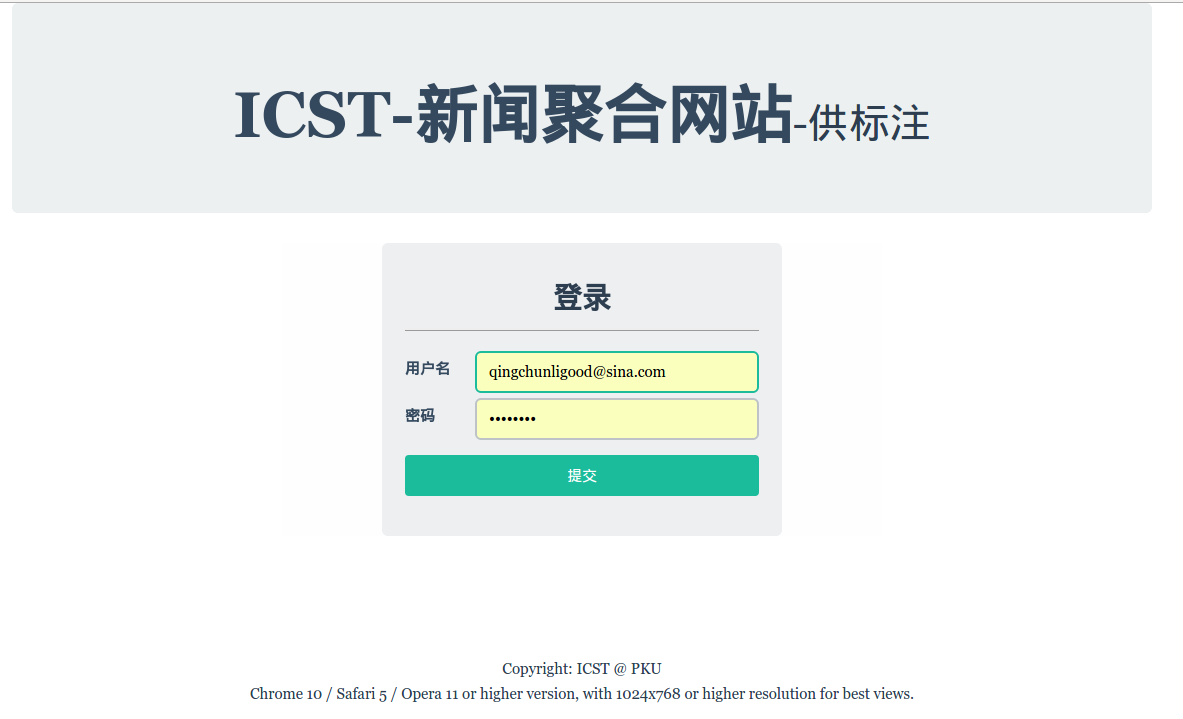
\includegraphics[width=0.9\hsize]{file/XNS_login.png}}
     \only<2-4>{
      \begin{overpic}[scale=.2]
	{file/XNS_HOME.png}
	\only<3,4>{\put(5,0){
	  \setlength{\fboxrule}{3pt} 
	  \setlength{\fboxsep}{0cm} 
	  \fbox{
\includegraphics[width=0.8\hsize]{file/XNS_board.png}} 
	}}
	\only<4>{\put(20,20){
	  \setlength{\fboxrule}{3pt} 
	  \setlength{\fboxsep}{0cm} 
	  \fbox{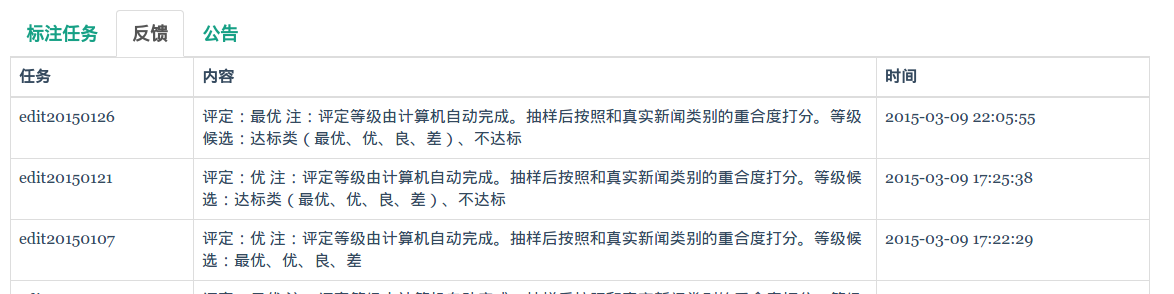
\includegraphics[width=0.8\hsize]{file/XNS_feedback.png}} 
	}}
      \end{overpic}
     }
     \only<5>{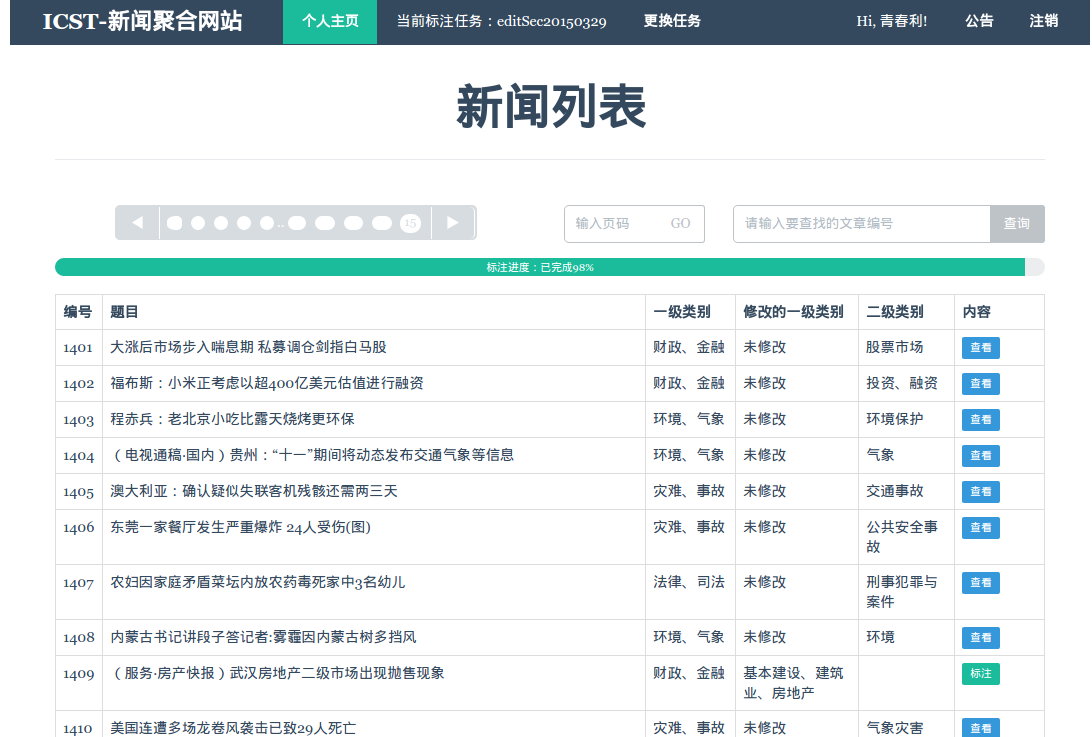
\includegraphics[width=0.9\hsize]{file/XNS_editList.png}}
     \only<6>{
\includegraphics[width=0.8\hsize]{file/XHS_editSec.png}}
     \only<7-8>{
      \begin{overpic}[scale=.2]
	{file/XNS_admin.png}
	\only<8>{\put(5,0){
	  \setlength{\fboxrule}{3pt} 
	  \setlength{\fboxsep}{0cm} 
	  \fbox{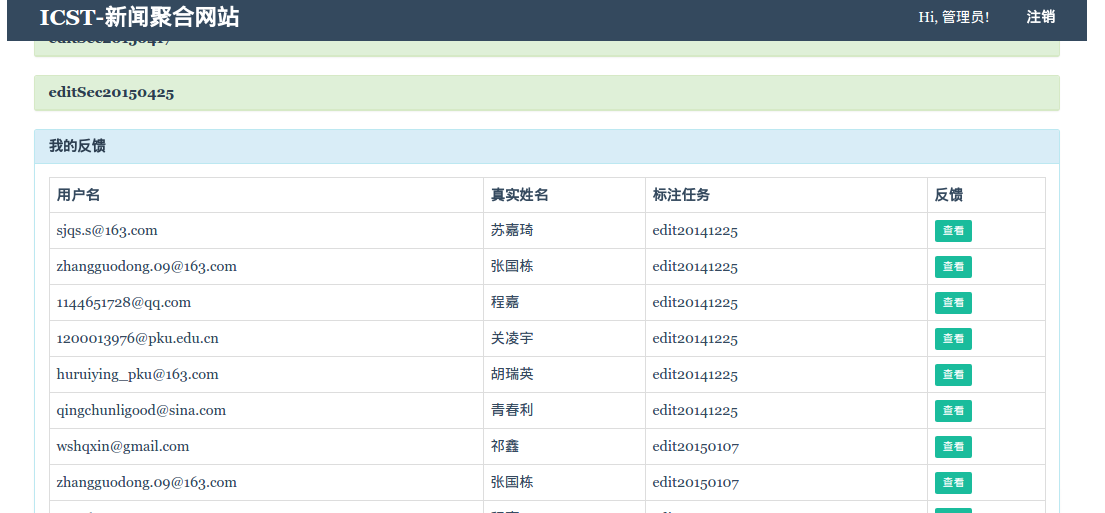
\includegraphics[width=0.8\hsize]{file/XNS_admin2.png}} 
	}}
      \end{overpic}
     }
    \end{columns}

}

\frame{
  \begin{columns}[c]
   \column{.15\hsize}
   \column{.7\hsize}
   \begin{block}{}
    \centering \Large 实验室工作 \\ 
    \small --- 中文维基百科谓词归一化
   \end{block}

   \column{.15\hsize}
  \end{columns}

}

\frame{
  \frametitle{实验室工作}
    \centering
    \begin{Large}
     中文维基百科谓词归一化
    \end{Large}
    
	\begin{figure}
	 \begin{minipage}[t]{0.2\linewidth}
	    \centering
	    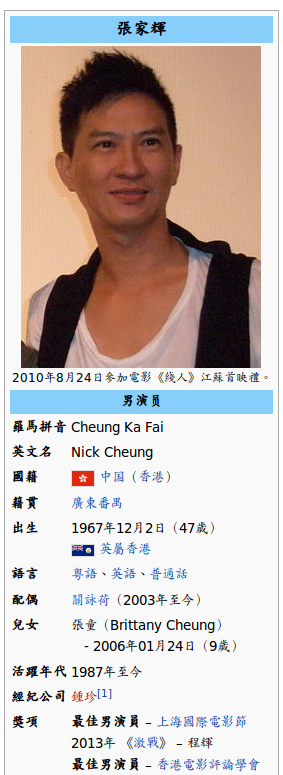
\includegraphics[width=0.8\textwidth]{file/张家辉.png}
	\end{minipage}
	\begin{minipage}[t]{0.5\linewidth}
	    \centering
	      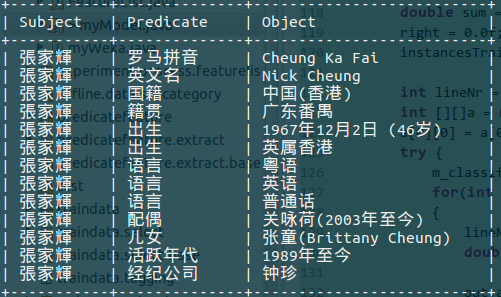
\includegraphics[width=1\linewidth]{file/张家辉mysql.png}
	\end{minipage}
       \end{figure}
   \begin{itemize}
    \item \red{背景/回顾}:基于中文维基百科的知识库:330w 三元组, 1.6w个谓词
   \end{itemize}
}

\frame{
  \frametitle{实验室工作}
    \centering
    \begin{Large}
     中文维基百科谓词归一化
    \end{Large}
    
    \begin{columns}{}
     \column{0.4\hsize}
    \begin{block}{"邮政"}
    INSEE/邮政编码、ISO 3166-2 邮政简写、美国邮政编号、美国邮政编码、邮政、邮政代码、邮政信箱、邮政分区、邮政区号
%     、邮政号码、邮政简称、邮政编号、邮政编号字母、邮政编码、邮政编码FSA、邮政编码首字母、邮政缩写
  \end{block}

     \column{0.6\hsize}
     \begin{itemize}
      \item Motivation:消除语义重复的谓词
      \item 问题转化:任给两个谓词,判断是否为相同语义
      \item 实验效果:在正负样本1:1的数据集上有监督训练,将近70\%的准确率
      \pause
      \item \textbf{进展}:投了NLPCC2015,被拒。。
     \end{itemize}

    \end{columns}

}

\frame{
  \frametitle{实验室工作}
    \centering
    \begin{Large}
     杂项
    \end{Large}
    
    \begin{columns}
     \column{0.1\hsize}
     
     \column{0.8\hsize}
     \begin{block}{}
      \begin{enumerate}
      \item 提供了NLPCC2015测评的知识库
	\begin{itemize}
	 \item NLPCC2015 task: Entity Recognition and Linking in Chinese Search Queries
	\end{itemize}
      \item 大组+小组讨论班 (报告4次)
     \end{enumerate}
     \end{block}
     \column{0.1\hsize}
    \end{columns}
}
\frame{
  \begin{columns}[c]
   \column{.15\hsize}
   \column{.7\hsize}
   \begin{block}{}
    \centering \Large 总结展望
   \end{block}

   \column{.15\hsize}
  \end{columns}

}

\frame{
  \frametitle{Summary}
  \begin{tikzpicture}
    \tikzstyle{Node}=[draw, rectangle, rounded corners, align=center]
    \node [Node, text width=2.5cm] (lastTerm) {
    \emph{上学期计划}
      \begin{itemize}\scriptsize
        \item 每日备忘录
        \item 每周两篇论文
        \item 考托福
      \end{itemize}

    } ;
    \node [Node, text width=4cm, right=of lastTerm] (thisTerm) {
      \emph{本学期完成}\scriptsize
      \begin{itemize}
       \item 每日备忘录
       \item 维基百科谓词的归一化
      \end{itemize}
    } ;
    
    \node [Node, text width=5cm, below=of lastTerm] (thisSummer) {
      \emph{暑期计划}
      \begin{footnotesize}
       \begin{itemize}\scriptsize
       \item 完善中文维基百科知识库的体系
	\begin{itemize}\scriptsize
	 \item 借鉴dbpedia,整合中英文维基百科、freebase
	\end{itemize}
       \item 看一下有关的书: shell,Java
       \item 修改NLPCC的论文,继续投稿
      \end{itemize}
      \end{footnotesize}
    };
    
    \node [Node, text width=4.5cm, right=of thisSummer] (nextTerm) {
      \emph{下学期计划}
      \begin{itemize}\scriptsize
       \item 尽量在开学时完成知识库体系构建,整理出一篇期刊
       \item 完成助教学分
       \item 百度百科的知识库提取和整合
       \item 动手做点小东西(展示知识库)
      \end{itemize}

    };
    
    \path[-Stealth, blue, thick] 
      (lastTerm) edge [bend left=10] (thisTerm) 
      (thisTerm) edge [bend left=10] (thisSummer) 
      (thisSummer) edge [bend left=10] (nextTerm) 
      ;
  \end{tikzpicture}

}

\frame{
  \begin{center}
   \Large 谢谢大家!
  \end{center}

}

\end{document}

